\documentclass[aspectratio=169,t,xcolor=table]{beamer}
\usepackage[utf8]{inputenc}

%\usepackage{multicol}
\usepackage{booktabs} 
\usepackage{subcaption}

\usetheme{Ufg}

%-------------------------------------theorems--------------
\newtheorem{conj}{Conjetura}
\newtheorem{defi}{Definição}
\newtheorem{teo}{Teorema}
\newtheorem{lema}{Lema}
\newtheorem{prop}{Proposição}
\newtheorem{cor}{Corolário}
\newtheorem{ex}{Exemplo}
\newtheorem{exer}{Exercício}

\setbeamertemplate{theorems}[numbered]
\setbeamertemplate{caption}[numbered]

%-------------------------------------------------------------%
%----------------------- Primary Definitions -----------------%

% This command set the default Color, is also possible to choose a custom color
\setPrimaryColor{UFGBlue} 


% -------------------------------------- Title Slide Information


\begin{document}
\title{Predicting Vehicle Loan Default}
\subtitle{Classification using the CRIF High Mark vehicle loan dataset}

\author{Paul Anderson\inst{1}\\Mike Barton\inst{1}\\Kevin Kincaid\inst{1}}

\institute[OSU] % (optional)
{
  \inst{1}%
   Data Analytics\\
  College of Science\\
  Oregon State University
}
\date{2026}
%-----------------------The next statement creates the title page.
\frame[noframenumbering]{\titlepage}



%---------------------------------------------------------Slide 2

\setLayout{horizontal} % Example of changing layout
%\setBGColor{Orange}  %Example of changing background color 


\begin{frame}{Data and Problem}
    \begin{columns}
        \column{0.33\textwidth}
        \textbf{Data}
        \begin{itemize}
        \item CRIF High Mark vehicle loan dataset
        \item n = 233,154
        \item Thin file: XXXX
        \item Normal: YYYY
        \end{itemize}
        
        \column{0.33\textwidth}
        \textbf{Classification Goal}
        \begin{itemize}
        \item Predict Defaults
        \end{itemize}
        
        \column{0.33\textwidth}
        \textbf{Tools}
        \begin{itemize}
            \item R: for EDA, cleaning, and modelling
        \end{itemize}
        
    \end{columns}
    \vspace{1cm}
 %\hrulefill
    \textbf{ Model Architectures Used}
    \vspace{.25cm}
    
    \begin{columns}
        \column{0.33\textwidth}
        Model 1: Random forest
        
        \column{0.33\textwidth}
        Model 2: XGBoost

    \end{columns}
    
\end{frame}
%---------------------------------------------------------




%---------------------------------------------------------Slide 3
\setLayout{vertical} % Example of changing layout
 

\begin{frame}{Findings: Random Forest Method}
    \begin{figure}
      \centering
      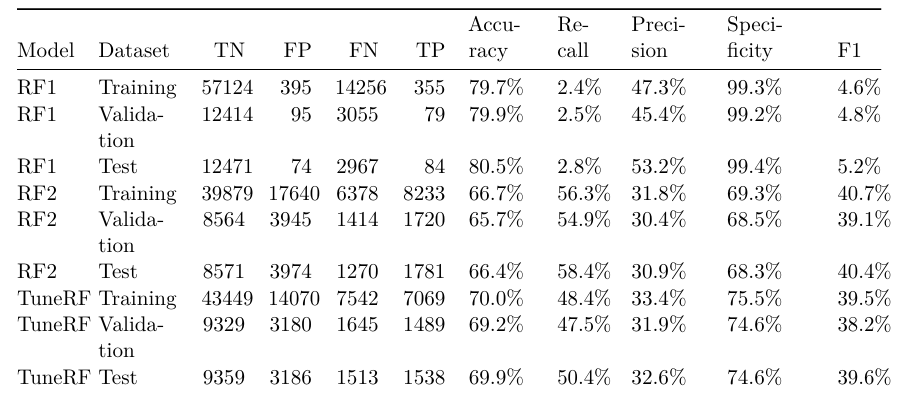
\includegraphics[width=0.8\textwidth]{figs/rf.png}
      \caption{Random Forest Model Accuracy}
      \label{fig:Random Forest Model Accuracy}
    \end{figure}
    
\end{frame}
%---------------------------------------------------------


%---------------------------------------------------------Slide 4


\begin{frame}{Findings: XGBoost Method}
    \begin{figure}
      \centering
      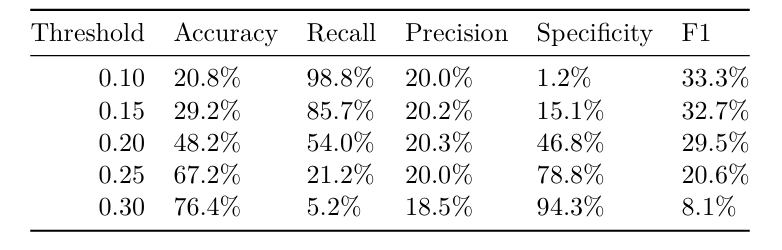
\includegraphics[width=0.9\textwidth]{figs/xgb.png}
      \caption{XGBoost Model Accuracy}
      \label{fig:XGBoost Model Accuracy}
    \end{figure}
    
\end{frame}
%---------------------------------------------------------


%---------------------------------------------------------Slide 5

\setLayout{blank}

\begin{frame}{Obstacles: Feature Engineering}
    \begin{columns}
    
        \column{0.4\textwidth}
        
        \textbf{The high dimensionality dataset had several complicated aspects to compensate for}
        \begin{itemize}
          \item Dimensionality Reduction
          \item High Cardinality Variables
          \item Creating stress score
        \end{itemize}
        
        \column{0.6\textwidth}
        \begin{figure}
          \centering
          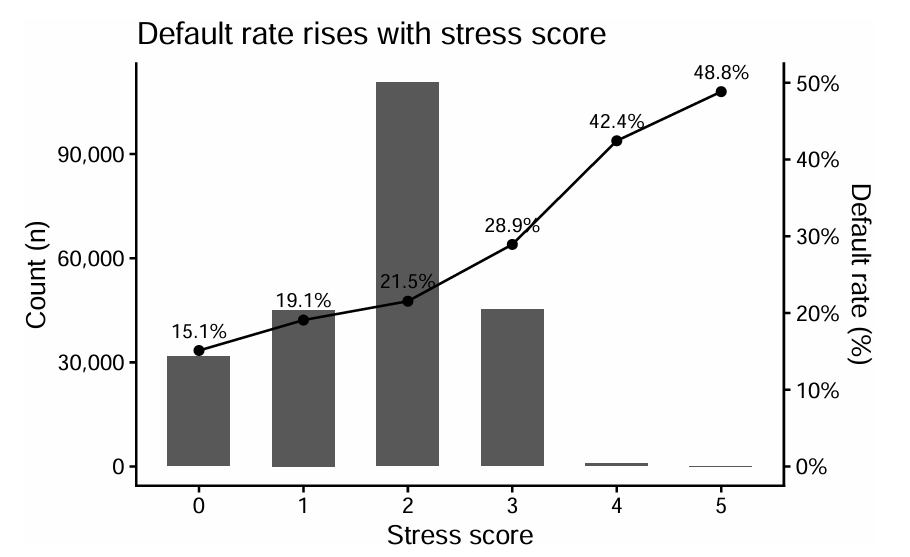
\includegraphics[width=.9\textwidth]{figs/stressscore.png}
          \caption{stress score.}
          \label{fig:stress score}
        \end{figure}
        
        
    \end{columns}
    
    \begin{columns}
    
    \end{columns}
    
\end{frame}
%---------------------------------------------------------


%---------------------------------------------------------Slide 6
\setLayout{vertical}

\begin{frame}{Obstacles: Imbalanced Categories}
    \textbf{Higher Proportion of Defaulted Observations}
    \begin{itemize}
      \item Different models performed better on a specific category
      \item XGBoost parameter adjustments
      \item SMOTE Methods
    \end{itemize}
    
\end{frame}
%---------------------------------------------------------



%---------------------------------------------------------Slide 7
\setLayout{horizontal}

\begin{frame}{Future Work}
    
    \text{Area 1: Further testing and refinement based on thin-normal file split}
    
    \text{Area 2: Utilizing a distributed cluster for faster calculation and better turning}
    
    \text{Area 3: Exploring greatly reduced model tuned to classification}
    
\end{frame}
%---------------------------------------------------------

%---------------------------------------------------------Slide 8
%Slide 10
%Thanks: Image of an Oregon City

\setLayout{blank} % Example of changing layout
\begin{frame}{Thanks}

%
\includegraphics[scale=0.5]{craterlake}

\end{frame}
%---------------------------------------------------------


\end{document}